\documentclass[11pt]{article}
\usepackage[utf8]{inputenc}
\usepackage{amsmath, amssymb, amsthm}
\usepackage{tikz}
\usetikzlibrary{automata, positioning, arrows.meta, shapes}
\usepackage{geometry}
\geometry{a4paper, margin=1in}

\title{Formal CSS Layout: FSM, Floats, and Inline Semantics}
\author{HTMLRules Formal Specification}
\date{December 2025}

\begin{document}

\maketitle

\section{Introduction}
This document formally specifies the CSS layout engine verified in Coq. It covers the Margin Collapsing FSM, the Floating Point model, and the Inline Formatting Context (IFC).

\section{1. Margin Collapsing FSM}
The vertical position of block boxes is governed by an accumulator machine dealing with adjacent margins $M$.

\subsection{Collapse Function (CSS 2.1 \S8.3.1)}
For a set of margins $M = \{m_1, \dots, m_n\}$:
\[ P = \{m \in M \mid m \ge 0\}, \quad N = \{m \in M \mid m < 0\} \]
\[ \text{Collapse}(M) = \max(\{0\} \cup P) + \min(\{0\} \cup N) \]

\section{2. Floating Point FSM}
Floating elements reduce the available horizontal space for normal flow content.

\subsection{State Definitions}
Let $\mathcal{L}$ and $\mathcal{R}$ be sets of rectangles (floats). The available horizontal interval $[L(y, h), R(y, h)]$ for a box of height $h$ at $y$ is:
\[ L(y, h) = \max \{ r.x + r.w \mid r \in \mathcal{L} \wedge \text{overlap}_y(r, y, h) \} \cup \{0\} \]
\[ R(y, h) = \min \{ r.x \mid r \in \mathcal{R} \wedge \text{overlap}_y(r, y, h) \} \cup \{W_{container}\} \]

\subsection{Placement Transition}
To place a float of size $(w, h)$, we find the minimal $y' \ge y_{current}$ such that:
\[ L(y', h) + w \le R(y', h) \]
The new state adds the rectangle to $\mathcal{L}$ or $\mathcal{R}$.

\section{3. Inline Formatting Context (IFC)}
Content flows horizontally into "line boxes" defined by the Float FSM.

\subsection{Line Wrapping Logic}
Given current state $(x, y)$ and next item $b$ with width $w_b$:
\begin{enumerate}
    \item \textbf{Check Fit}: Let range be $[l, r] = \text{Range}(y, h_{line})$.
    \item \textbf{If} $x + w_b \le r$: Place at $x$, $x_{new} = x + w_b$.
    \item \textbf{Else}: New Line. $y_{new} = y + h_{line}$, $x_{new} = L(y_{new}, h_b)$.
\end{enumerate}

\section{System Diagram}
\begin{center}
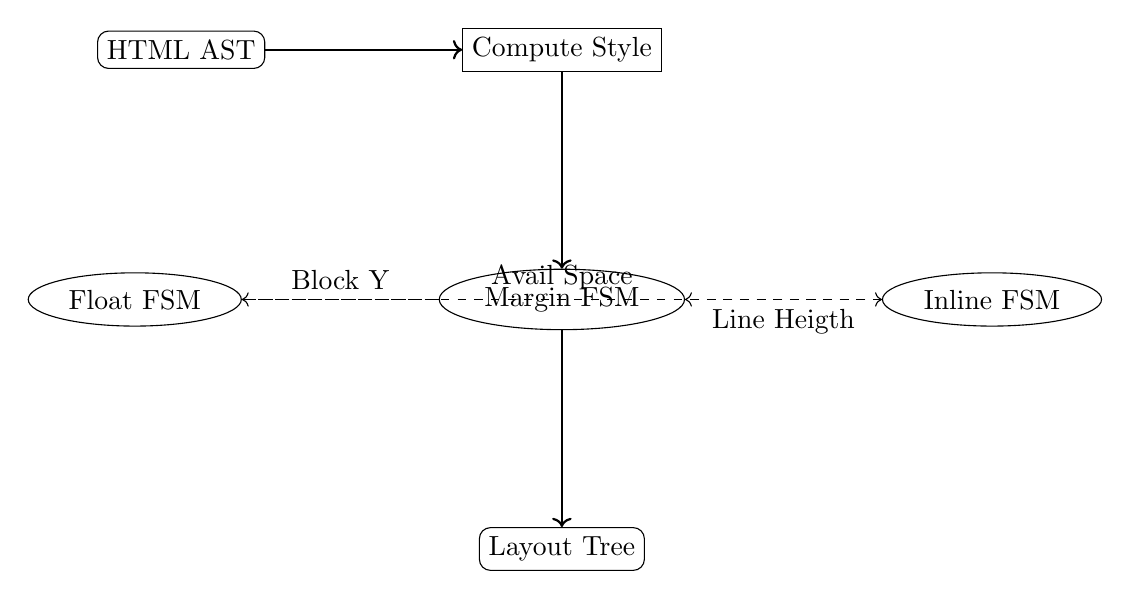
\begin{tikzpicture}[node distance=2.5cm, auto]
    % Nodes
    \node[draw, rectangle, rounded corners] (Input) {HTML AST};
    \node[draw, rectangle, right=of Input] (Style) {Compute Style};
    \node[draw, ellipse, below=of Style] (MarginFSM) {Margin FSM};
    \node[draw, ellipse, left=of MarginFSM] (FloatFSM) {Float FSM};
    \node[draw, ellipse, right=of MarginFSM] (InlineFSM) {Inline FSM};
    \node[draw, rectangle, rounded corners, below=of MarginFSM] (Layout) {Layout Tree};

    % Paths
    \path[->, thick] (Input) edge (Style);
    \path[->, thick] (Style) edge (MarginFSM);
    
    \path[->, dashed] (MarginFSM) edge node[above] {Block Y} (FloatFSM);
    \path[->, dashed] (FloatFSM) edge node[above] {Avail Space} (InlineFSM);
    \path[->, dashed] (InlineFSM) edge node[below] {Line Heigth} (MarginFSM);
    
    \path[->, thick] (MarginFSM) edge (Layout);
\end{tikzpicture}
\end{center}

\section{Transition Diagram}
\begin{center}
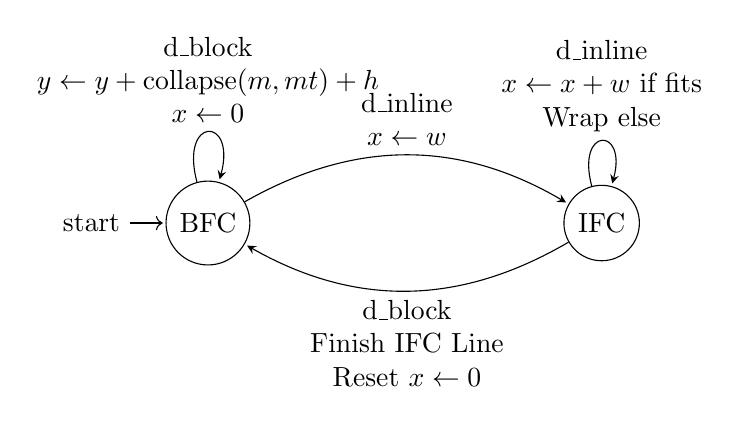
\begin{tikzpicture}[shorten >=1pt, node distance=5cm, on grid, auto]
    \node[state, initial] (BFC) {BFC};
    \node[state, right=of BFC] (IFC) {IFC};
    
    \path[->, >=stealth]
        (BFC) edge [loop above] node [align=center] {d\_block\\$y \gets y + \text{collapse}(m, mt) + h$\\$x \gets 0$} (BFC)
        (BFC) edge [bend left] node [align=center] {d\_inline\\$x \gets w$} (IFC)
        (IFC) edge [bend left] node [align=center] {d\_block\\Finish IFC Line\\Reset $x \gets 0$} (BFC)
        (IFC) edge [loop above] node [align=center] {d\_inline\\$x \gets x + w$ if fits\\Wrap else} (IFC);
\end{tikzpicture}
\end{center}

\end{document}
